\begin{landscape}
	\begin{figure}[htb]
		\centering
	%	\begin{adjustwidth}{-0.2\linewidth}{-0.2\linewidth}
	%		\hspace{+20pt}
			\begin{subfigure}[c]{.45\linewidth}
				\centering
				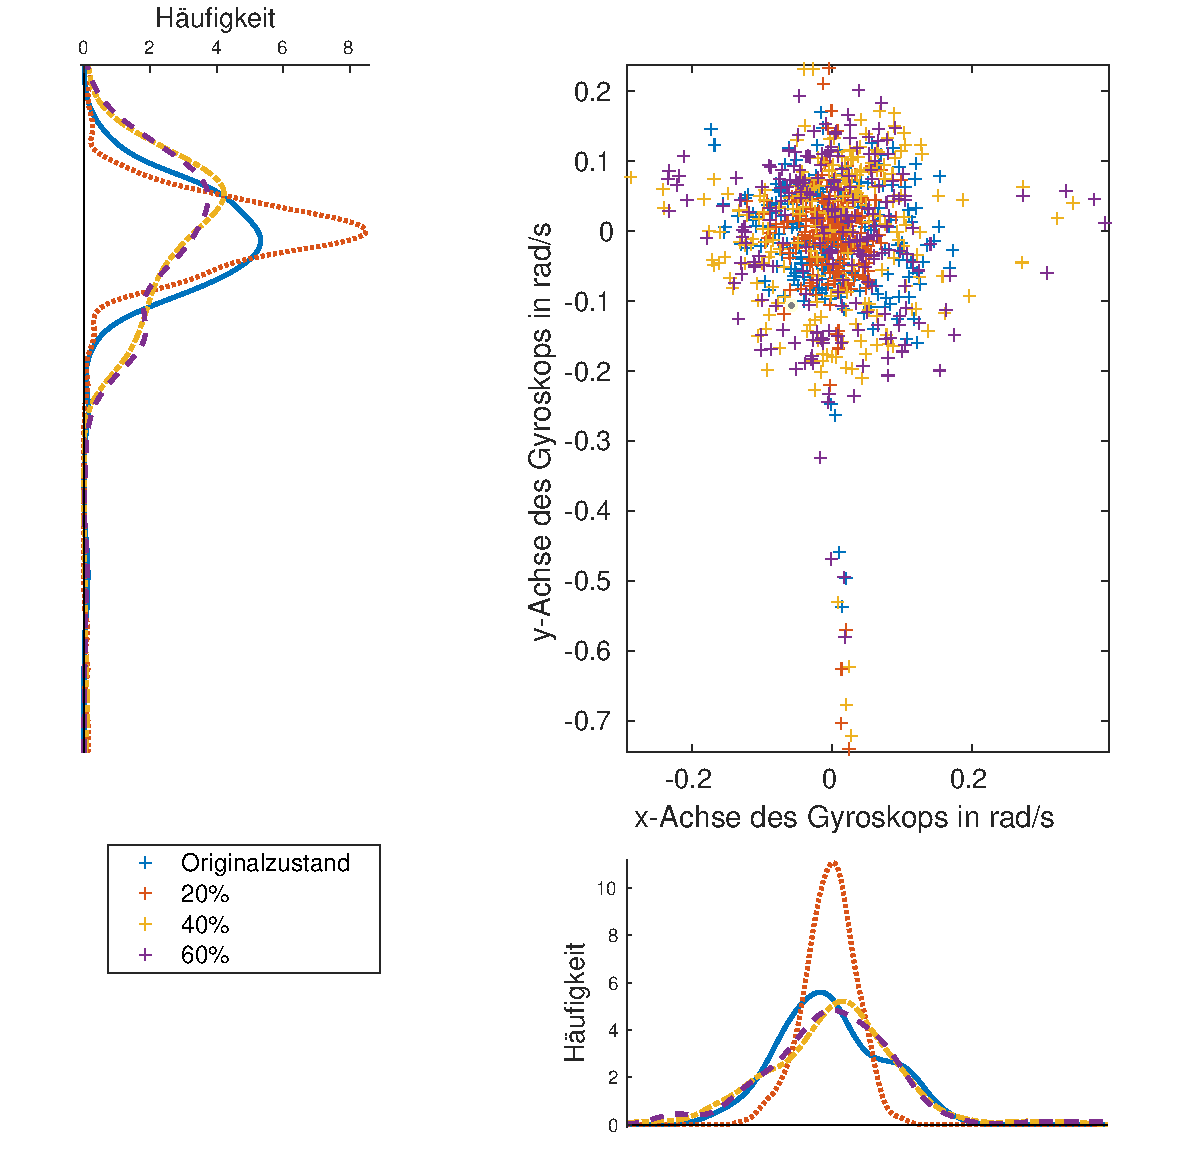
\includegraphics[width=\linewidth]{Bilder/Gyr_Grund_20_40_60_ohneM.pdf}
				\caption{ohne Magneten} \label{Gyr_ohne}
%				\vspace{5pt}
			\end{subfigure}
			\hfill
	%		\hspace{-35pt}
			\begin{subfigure}[c]{.45\linewidth}
				\centering
				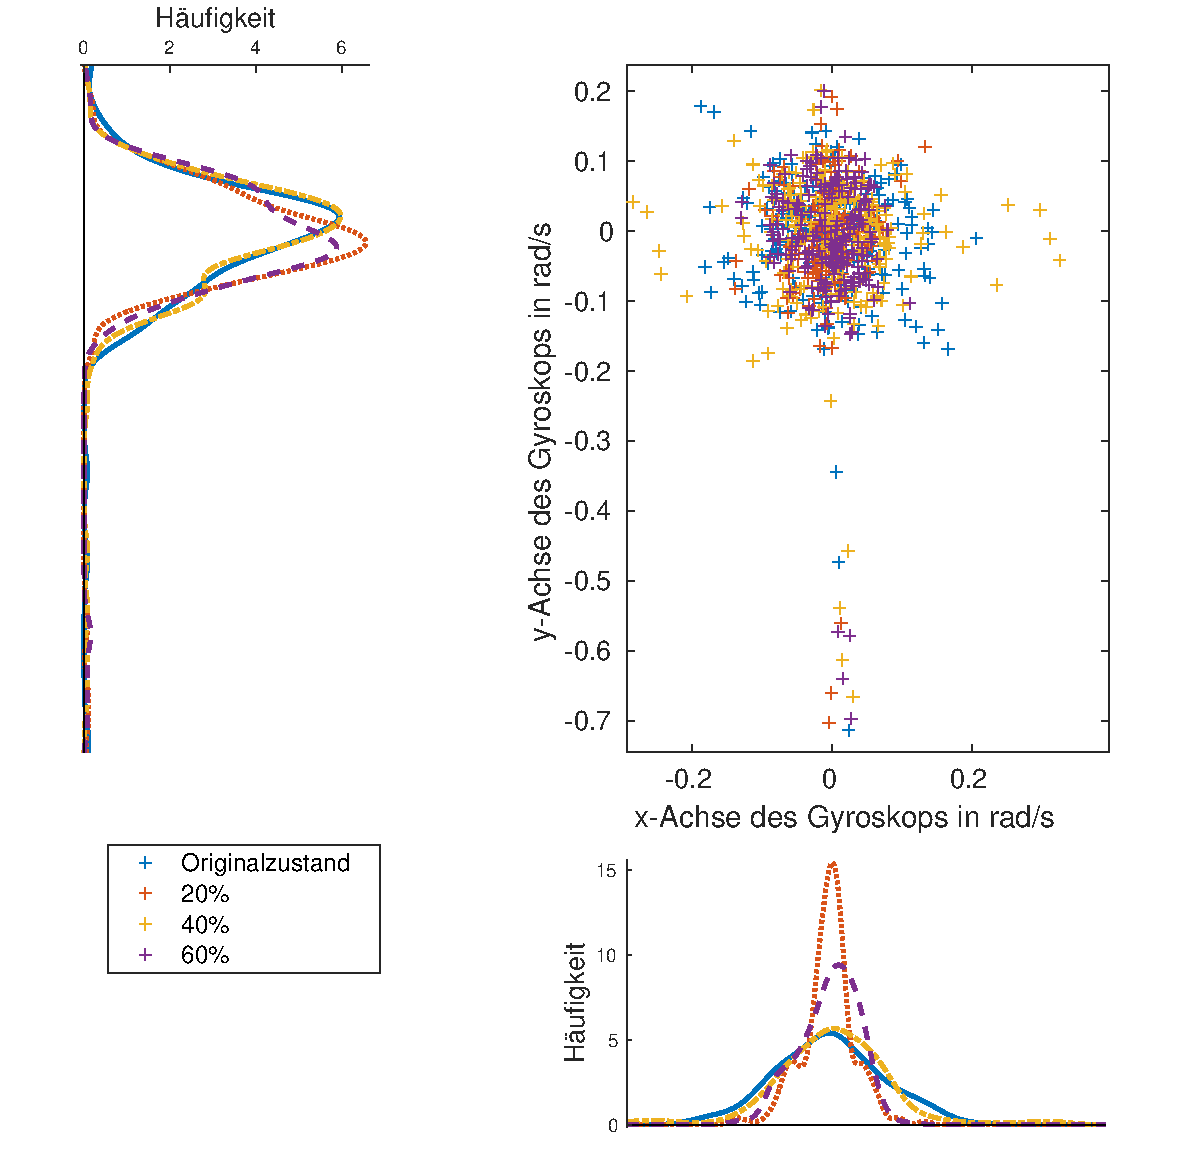
\includegraphics[width=\linewidth]{Bilder/Gyr_Grund_20_40_60_mitM.pdf}
				\caption{mit Magneten} \label{Gyr_mit}
%				\vspace{5pt}
			\end{subfigure}
	%	\end{adjustwidth}
		\caption{Ausgabe des Gyroskops, x-Achse auf y-Achse mit jeweiliger Wahrscheinlichkeitsdichtefunktion}\label{Gyr}
	\end{figure}
\end{landscape}